\section{空间解析几何 III}

\subsection{柱面}

\begin{definition}[柱面]
	平行于指定直线的直线 $L$ 沿一条空间曲线 $C$ 移动形成的曲面称为\textbf{柱面}。这条定曲线 $C$ 称为柱面的\textbf{准线}，动直线 $L$ 称为柱面的\textbf{母线}。
\end{definition}

一般而言，方程 $F(x, y) = 0$ 表示空间中母线平行于 $z$ 轴的一个柱面，其准线是 $xOy$ 面上的曲线 $C: F(x, y) = 0$。其它坐标轴同理。

\subsection{二次曲面}

\begin{definition}[二次曲面]
	三元二次方程 $F(x, y, z) = 0$ 表示的曲面称为\textbf{二次曲面}。
\end{definition}

\subsubsection{椭圆锥面}

方程形如 $\frac{x^2}{a^2} + \frac{y^2}{b^2} = z^2$ 的曲面称为\textbf{椭圆锥面}。

\begin{figure}[H]
	\centering
	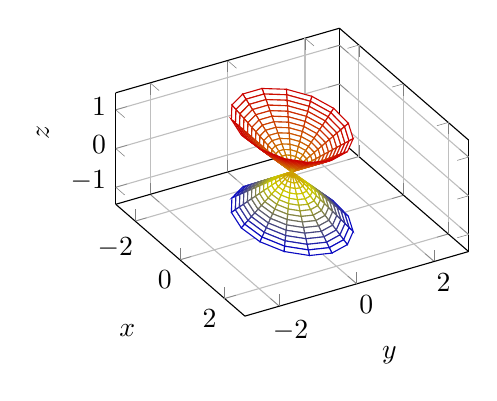
\begin{tikzpicture}
		\pgfplotsset{compat=1.18}
		\begin{axis}[
			axis equal,
			width=0.5\textwidth,
			view={60}{30},
			xlabel={$x$}, ylabel={$y$}, zlabel={$z$},
			grid=major,
			z buffer=sort
		]
		\addplot3[surf, fill=white, draw=black, samples=16, domain=0:1.2, y domain=0:360]
			({1.5*x*cos(y)}, {x*sin(y)}, {x});
		\addplot3[surf, fill=white, draw=black, samples=16, domain=0:1.2, y domain=0:360]
			({1.5*x*cos(y)}, {x*sin(y)}, {-x});
		\end{axis}
	\end{tikzpicture}
	\caption{椭圆锥面}
\end{figure}

每一个 $z = t$ 平面截该曲面会得到一族相似的椭圆，且椭圆的轴长随 $z$ 线性变化。

\subsubsection{椭球面}

方程形如 $\frac{x^2}{a^2} + \frac{y^2}{b^2} + \frac{z^2}{c^2} = 1$ 的曲面称为\textbf{椭球面}。

\begin{figure}[H]
	\centering
	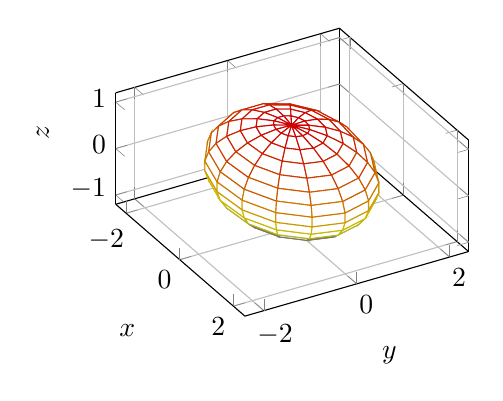
\begin{tikzpicture}
		\begin{axis}[
			axis equal,
			width=0.5\textwidth,
			view={60}{30},
			xlabel={$x$}, ylabel={$y$}, zlabel={$z$},
			grid=major,
			z buffer=sort
		]
		\addplot3[surf, fill=white, draw=black, samples=16, domain=0:180, y domain=0:360]
			({2*sin(x)*cos(y)}, {1.5*sin(x)*sin(y)}, {cos(x)});
		\end{axis}
	\end{tikzpicture}
	\caption{椭球面}
\end{figure}

椭球面是球面经过伸缩变换得到的。

\subsubsection{单叶双曲面}

方程形如 $\frac{x^2}{a^2} + \frac{y^2}{b^2} - \frac{z^2}{c^2} = 1$ 的曲面称为\textbf{单叶双曲面}。

\begin{figure}[H]
	\centering
	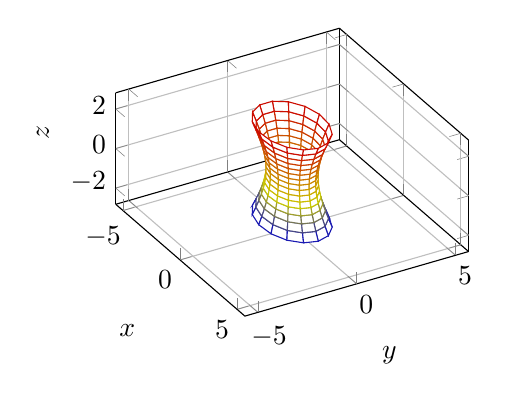
\begin{tikzpicture}
		\begin{axis}[
			axis equal,
			width=0.5\textwidth,
			view={60}{30},
			xlabel={$x$}, ylabel={$y$}, zlabel={$z$},
			grid=major,
			z buffer=sort
		]
		\addplot3[surf, fill=white, draw=black, samples=16, domain=-1:1, y domain=0:360]
			({1.5*cosh(x)*cos(y)}, {cosh(x)*sin(y)}, {2*sinh(x)});
		\end{axis}
	\end{tikzpicture}
	\caption{单叶双曲面}
\end{figure}

单叶双曲面是由 $xOz$ 上的双曲线 $\frac{x^2}{a^2} - \frac{z^2}{c^2} = 1$ 绕 $z$ 轴旋转，得到旋转单叶双曲面 $\frac{x^2 + y^2}{a^2} - \frac{z^2}{c^2} = 1$，再经过伸缩变换得到的。

\subsubsection{双叶双曲面}

方程形如 $\frac{x^2}{a^2} - \frac{y^2}{b^2} - \frac{z^2}{c^2} = 1$ 的曲面称为\textbf{双叶双曲面}。

\begin{figure}[H]
	\centering
	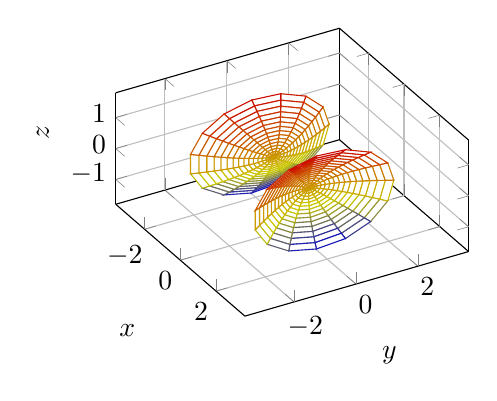
\begin{tikzpicture}
		\begin{axis}[
			axis equal,
			width=0.5\textwidth,
			view={60}{30},
			xlabel={$x$}, ylabel={$y$}, zlabel={$z$},
			grid=major,
			z buffer=sort
		]
		\addplot3[surf, fill=white, draw=black, samples=16, domain=0:1.2, y domain=0:360]
			({-cosh(x)}, {1.5*sinh(x)*cos(y)}, {sinh(x)*sin(y)});
		\addplot3[surf, fill=white, draw=black, samples=16, domain=0:1.2, y domain=0:360]
			({cosh(x)}, {1.5*sinh(x)*cos(y)}, {sinh(x)*sin(y)});
		\end{axis}
	\end{tikzpicture}
	\caption{双叶双曲面}
\end{figure}

与单叶类似，但是是由 $xOz$ 上的双曲线 $\frac{x^2}{a^2} - \frac{z^2}{c^2} = 1$ 绕 $x$ 轴旋转、伸缩得到的。

\subsubsection{椭圆抛物面}

方程形如 $\frac{x^2}{a^2} + \frac{y^2}{b^2} = z$ 的曲面称为\textbf{椭圆抛物面}。

\begin{figure}[H]
	\centering
	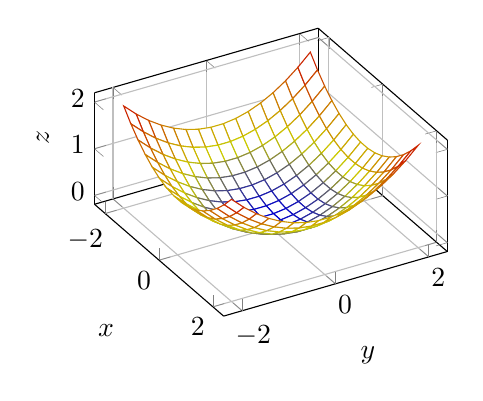
\begin{tikzpicture}
		\begin{axis}[
			axis equal,
			width=0.5\textwidth,
			view={60}{30},
			xlabel={$x$}, ylabel={$y$}, zlabel={$z$},
			grid=major,
			z buffer=sort
		]
		\addplot3[surf, fill=white, draw=black, samples=16, domain=-2:2, y domain=-2:2]
			{x^2/4 + y^2/4};
		\end{axis}
	\end{tikzpicture}
	\caption{椭圆抛物面}
\end{figure}

椭圆抛物面是 $xOz$ 面上的抛物线 $\frac{x^2}{a^2} = z$ 绕 $z$ 轴旋转得到旋转抛物面，再进行伸缩变换得到的。

\subsubsection{双曲抛物面}

方程形如 $\frac{x^2}{a^2} - \frac{y^2}{b^2} = z$ 的曲面称为\textbf{双曲抛物面}，又称为\textbf{马鞍面}。

用 $x = t$ 截该曲面，得到截痕 $l$ 为平面 $x = t$ 上的抛物线 $-\frac{y^2}{b^2} = z - \frac{t^2}{a^2}$，其顶点坐标为 $\ab(t, 0, \frac{t^2}{a^2})$。也就是说，双曲抛物面是由 $yOz$ 面上的抛物线 $l$，沿着 $xOz$ 面上另一个抛物线 $L: z = \frac{x^2}{a^2}$ 平移得到的曲面。

\begin{figure}[H]
	\centering
	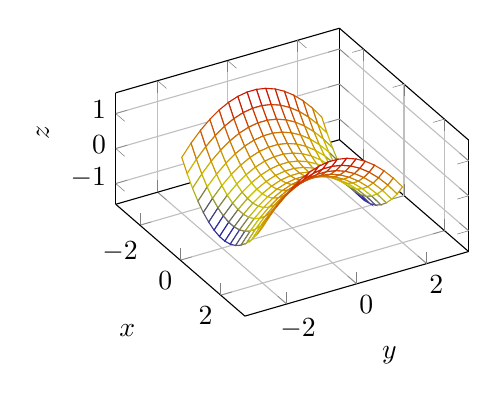
\begin{tikzpicture}
		\begin{axis}[
			axis equal,
			width=0.5\textwidth,
			view={60}{30},
			xlabel={$x$}, ylabel={$y$}, zlabel={$z$},
			grid=major,
			z buffer=sort
		]
		\addplot3[surf, fill=white, draw=black, samples=16, domain=-2:2, y domain=-2:2]
			{x^2/3 - y^2/3};
		\end{axis}
	\end{tikzpicture}
	\caption{双曲抛物面}
\end{figure}

\subsection{作业}

\begin{problem}
	习题 8.5.2
	\begin{solution}
		$$
		(x - 1)^2 + (y - 3)^2 + (z + 2)^2 = 14
		$$
	\end{solution}
\end{problem}

\begin{problem}
	习题 8.5.3
	\begin{solution}
		化简：
		$$
		(x - 2)^2 + (y + 2)^2 + (z + 1)^2 = 9
		$$
		因此这是一个球面。
	\end{solution}
\end{problem}

\begin{problem}
	习题 8.5.4
	\begin{solution}
		设 $P(2, 3, 4)$。根据平面几何知识可知，对于每个过 $OP$ 连线的平面上，满足题意的点都构成一个圆。因此这是一个球面。
	\end{solution}
\end{problem}

\begin{problem}
	习题 8.5.5
	\begin{solution}
		$$
		y^2 + z^2 = 5x
		$$
	\end{solution}
\end{problem}

\begin{problem}
	习题它 8.5.6
	\begin{solution}
		$$
		x^2 + y^2 + z^2 = 9
		$$
	\end{solution}
\end{problem}

\begin{problem}
	习题 8.5.8
	\begin{solution}
		\begin{enumerate}
			\item[\textbf{1)}] 这是一个母线为 $z$ 轴的圆柱面；
			\item[\textbf{2)}] 这是一个母线为 $z$ 轴的双曲柱面；
			\item[\textbf{3)}] 这是一个母线为 $y$ 轴的椭圆柱面；
			\item[\textbf{4)}] 这是一个母线为 $x$ 轴的抛物柱面；
			\item[\textbf{5)}] 这是一个母线为 $y$ 轴的抛物柱面。
			
			\begin{figure}[H]
				\centering
				% 第一行：图1 和 图2
				\begin{subfigure}[b]{0.45\textwidth}
					\centering
					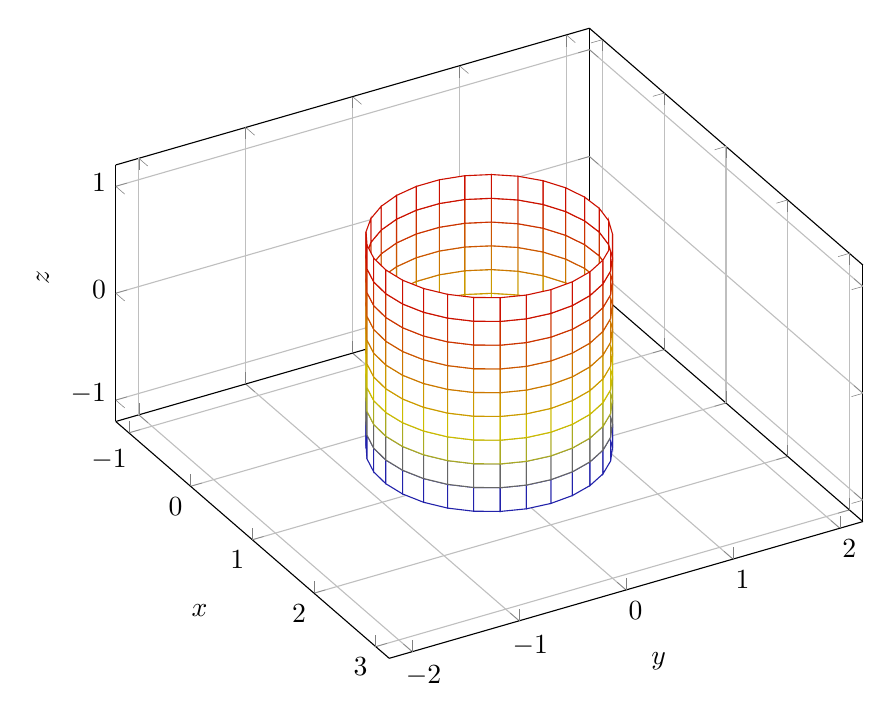
\begin{tikzpicture}
					\begin{axis}[
						scale=0.9,
						axis equal,
						width=\textwidth, % 自适应子图宽度
						view={60}{30},
						xlabel=$x$, ylabel=$y$, zlabel=$z$,
						grid=major
					]
					\addplot3[
						surf,
						fill=white, draw=black,
						domain=0:360,
						y domain=-1:1,
						samples=30,
						samples y=10
					]
					({1 + cos(x)}, {sin(x)}, {y});
					\end{axis}
					\end{tikzpicture}
					\caption{$(x-1)^2 + y^2 = 1$}
				\end{subfigure}
				\hfill % 两图之间填充空白
				\begin{subfigure}[b]{0.45\textwidth}
					\centering
					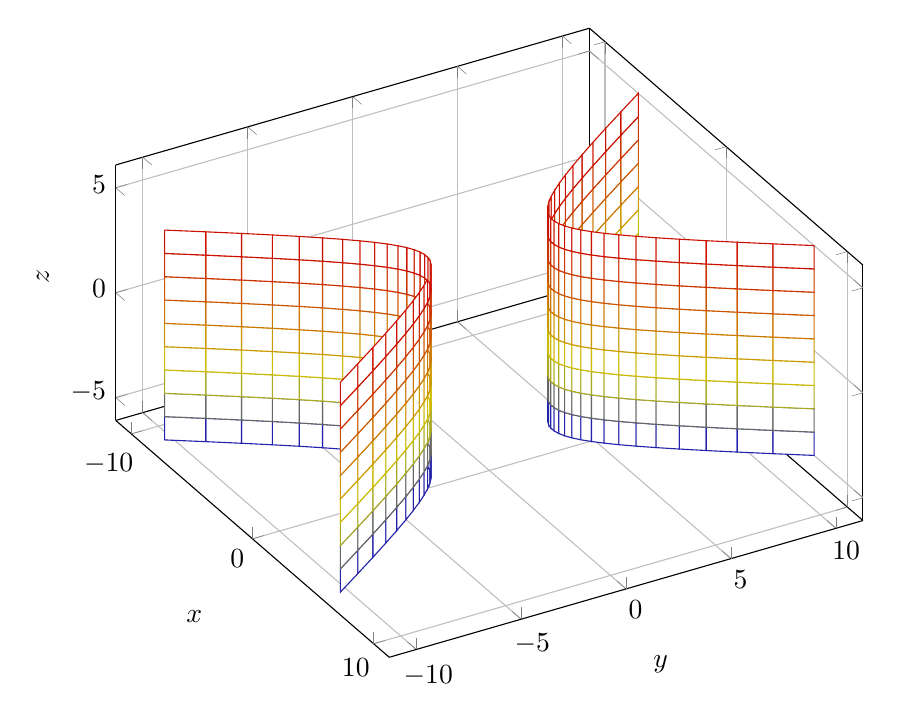
\begin{tikzpicture}
					\begin{axis}[
						scale=0.9,
						axis equal,
						width=\textwidth,
						view={60}{30},
						xlabel=$x$, ylabel=$y$, zlabel=$z$,
						grid=major
					]
					\addplot3[
						surf,
						fill=white, draw=black,
						domain=-2:2,
						y domain=-5:5,
						samples=30,
						samples y=10
					]
					({2*sinh(-x)}, {-3*cosh(-x)}, {-y});
					\addplot3[
						surf,
						fill=white, draw=black,
						domain=-2:2,
						y domain=-5:5,
						samples=30,
						samples y=10
					]
					({2*sinh(x)}, {3*cosh(x)}, {y});
					\end{axis}
					\end{tikzpicture}
					\caption{$-\frac{x^2}{4} + \frac{y^2}{9} = 1$}
				\end{subfigure}
			\end{figure}

			\begin{figure}[H]
				\centering
				% 第二行：图3 和 图4
				\begin{subfigure}[b]{0.45\textwidth}
					\centering
					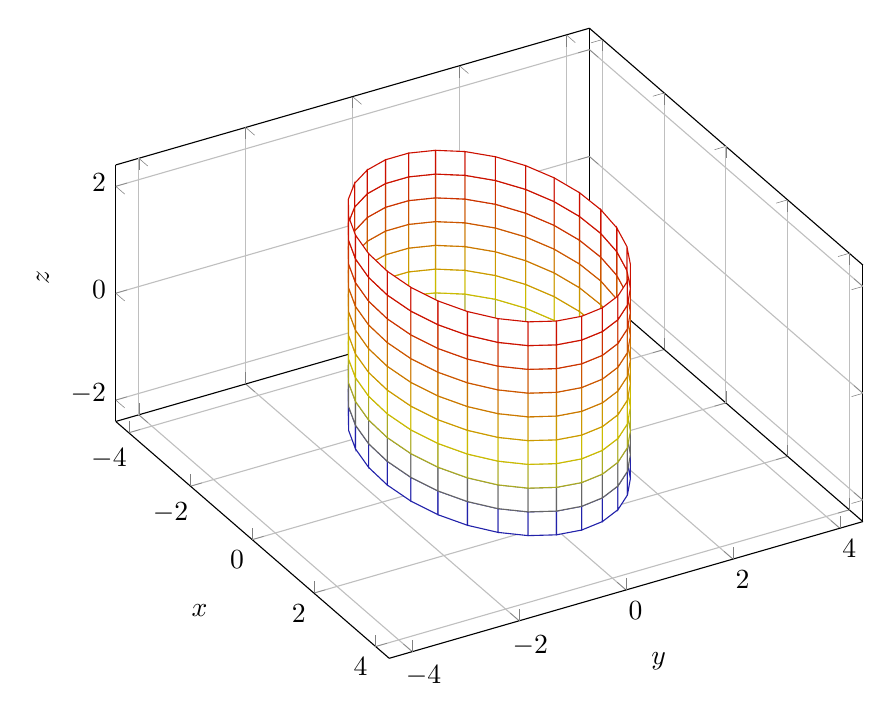
\begin{tikzpicture}
					\begin{axis}[
						scale=0.9,
						axis equal,
						width=\textwidth,
						view={60}{30},
						xlabel=$x$, ylabel=$y$, zlabel=$z$,
						grid=major
					]
					\addplot3[
						surf,
						fill=white, draw=black,
						domain=0:360,
						y domain=-2:2,
						samples=30,
						samples y=10,
					]
					({3*cos(x)}, {2*sin(x)}, {y});
					\end{axis}
					\end{tikzpicture}
					\caption{$\frac{x^2}{9} + \frac{y^2}{4} = 1$}
				\end{subfigure}
				\hfill
				\begin{subfigure}[b]{0.45\textwidth}
					\centering
					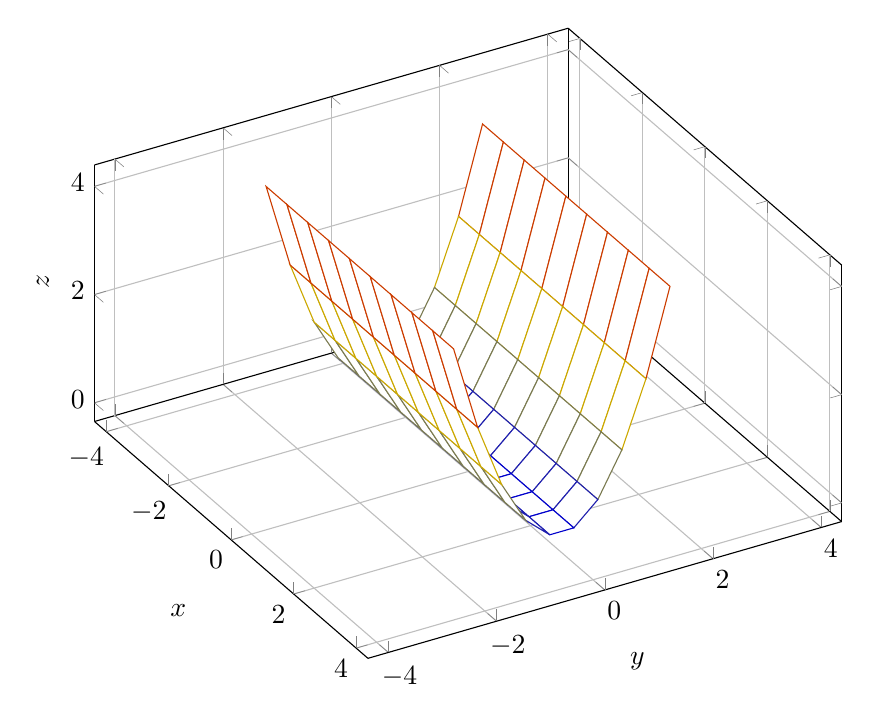
\begin{tikzpicture}
					\begin{axis}[
						scale=0.9,
						axis equal,
						width=\textwidth,
						view={60}{30},
						xlabel=$x$, ylabel=$y$, zlabel=$z$,
						grid=major
					]
					\addplot3[
						surf,
						fill=white, draw=black,
						domain=-3:3,
						y domain=-2:2,
						samples=10,
					]
					{y^2};
					\end{axis}
					\end{tikzpicture}
					\caption{$z = y^2$}
				\end{subfigure}
			\end{figure}

			\begin{figure}[H]
				\centering
				% 第三行：图5（居中）
				\begin{subfigure}[b]{0.45\textwidth}
					\centering
					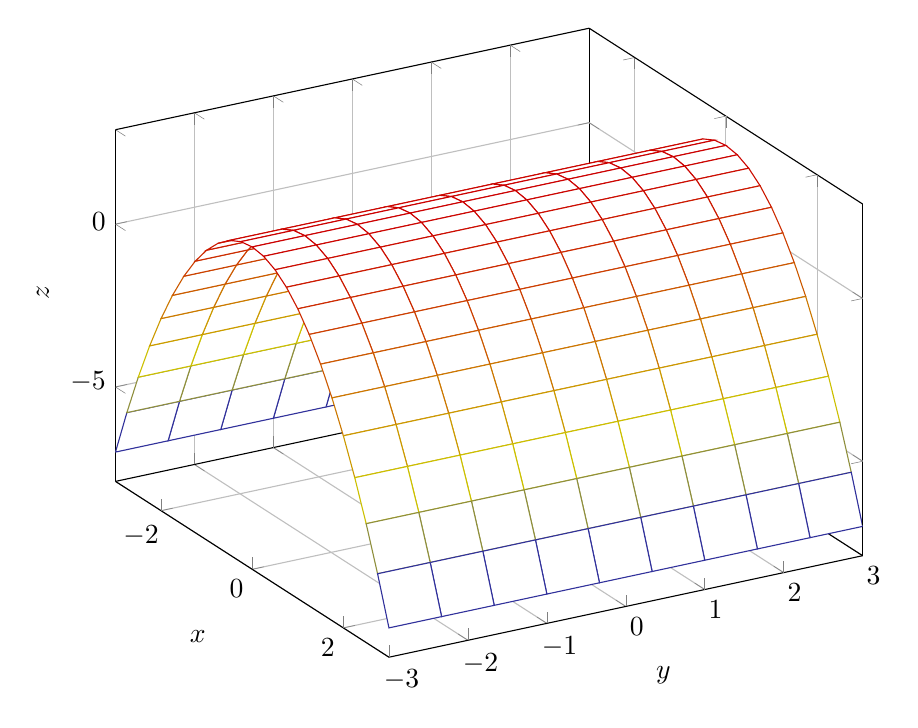
\begin{tikzpicture}
					\begin{axis}[
						scale=0.9,
						width=\textwidth,
						view={60}{30},
						xlabel=$x$, ylabel=$y$, zlabel=$z$,
						grid=major
					]
					\addplot3[
						surf,
						fill=white, draw=black,
						domain=-3:3,
						y domain=-3:3,
						samples=25,
						samples y=10
					]
					{2 - x^2};
					\end{axis}
					\end{tikzpicture}
					\caption{$z = 2 - x^2$}
				\end{subfigure}
			\end{figure}
		\end{enumerate}
	\end{solution}
\end{problem}

\begin{problem}
	习题 8.5.9
	\begin{solution}
		\begin{enumerate}
			\item[\textbf{1)}] 平面解析几何中这是一条直线，空间解析几何中这是一个平面；
			\item[\textbf{2)}] 平面解析几何中这是一条直线，空间解析几何中这是一个平面；
			\item[\textbf{3)}] 平面解析几何中这是一个圆，空间解析几何中这是一个圆柱面；
			\item[\textbf{4)}] 平面解析几何中这是一条双曲线，空间解析几何中这是一个双曲柱面。
		\end{enumerate}
	\end{solution}
\end{problem}

\begin{problem}
	习题 8.5.11
	\begin{solution}
		\begin{enumerate}
			\item[\textbf{1)}] 这是一个单叶双曲面；
			\item[\textbf{2)}] 这是一个双叶双曲面；
			\item[\textbf{3)}] 这是一个椭圆抛物面。
		\end{enumerate}

		\begin{figure}[H]
			\centering
			\begin{subfigure}[b]{0.45\textwidth}
				\centering
				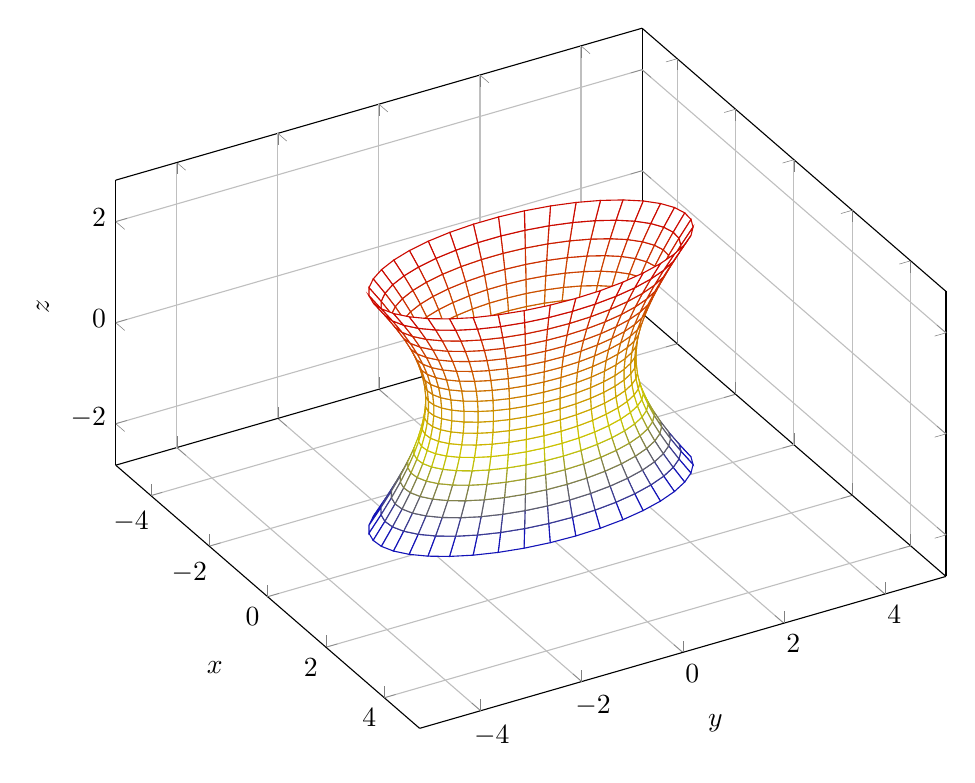
\begin{tikzpicture}
				\begin{axis}[
					axis equal,
					width=\textwidth,
					view={60}{30},
					xlabel={$x$}, ylabel={$y$}, zlabel={$z$},
					grid=major,
					z buffer=sort,
				]
				\addplot3 [
					surf,
					fill=white,
					draw=black,
					domain=0:360,
					domain y=-1:1,
					samples=40,
					samples y=20
				]
				({cosh(y)*cos(x)}, {2*cosh(y)*sin(x)}, {2*sinh(y)});
				\end{axis}
				\end{tikzpicture}
				\caption{$4x^2 + y^2 - z^2 = 4$}
			\end{subfigure}
			\hfill
			\begin{subfigure}[b]{0.45\textwidth}
				\centering
				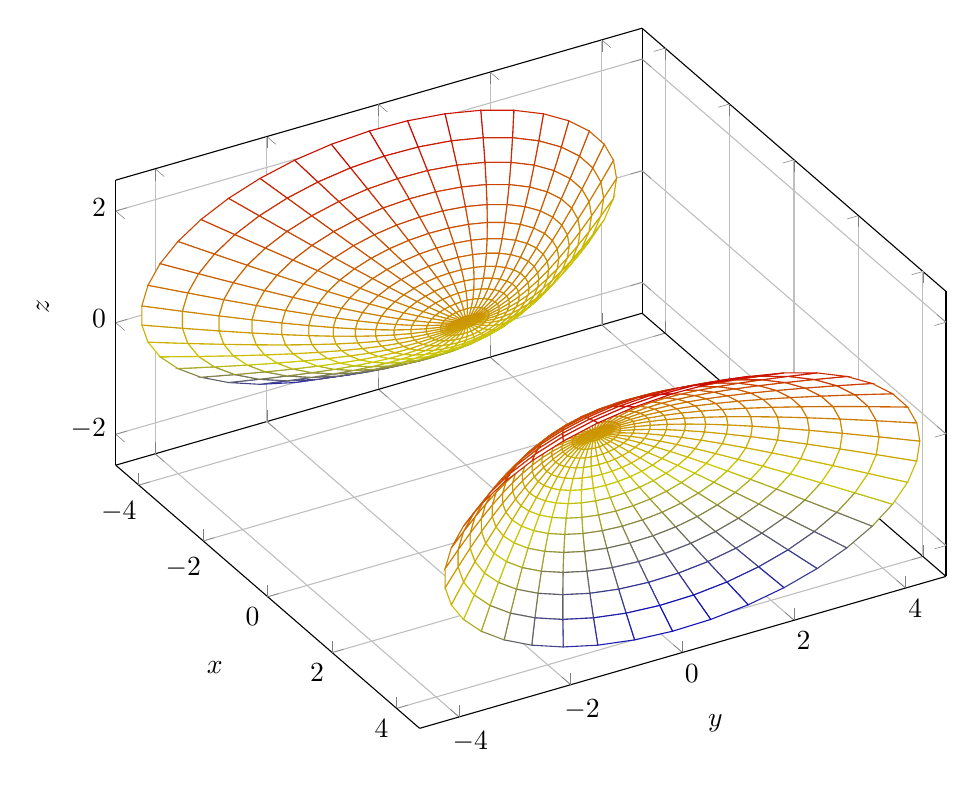
\begin{tikzpicture}
				\begin{axis}[
					axis equal,
					width=\textwidth,
					view={60}{30},
					xlabel={$x$}, ylabel={$y$}, zlabel={$z$},
					grid=major,
					z buffer=sort
				]
				\addplot3 [
					surf, 
					fill=white,
					draw=black,
					domain=0:360,
					domain y=0:1.5,
					samples=40,
					samples y=15
				]
				({2*cosh(y)}, {2*sinh(y)*cos(x)}, {sinh(y)*sin(x)});
				\addplot3 [
					surf, 
					fill=white,
					draw=black,
					domain=0:360,
					domain y=0:1.5,
					samples=40,
					samples y=15
				]
				({-2*cosh(y)}, {2*sinh(y)*cos(x)}, {sinh(y)*sin(x)});
				\end{axis}
				\end{tikzpicture}
				\caption{$x^2 - y^2 - 4z^2 = 4$}
			\end{subfigure}
			\vspace{2ex}
			\begin{subfigure}[b]{0.45\textwidth}
				\centering
				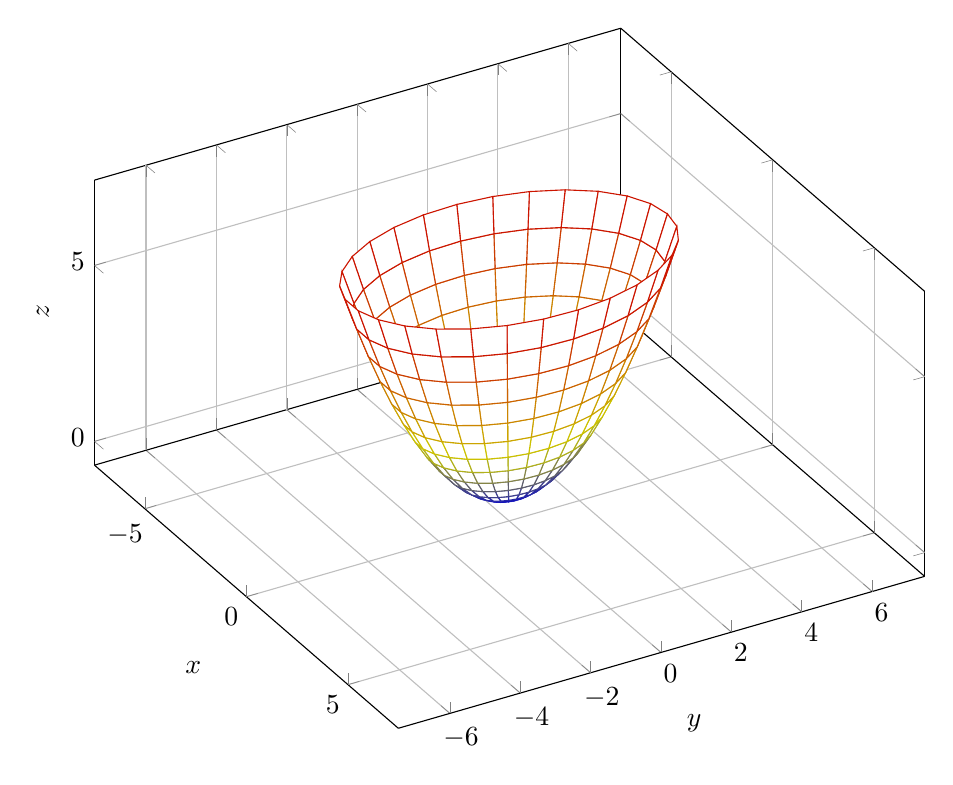
\begin{tikzpicture}
				\begin{axis}[
					axis equal,
					width=\textwidth,
					view={60}{30},
					xlabel={$x$}, ylabel={$y$}, zlabel={$z$},
					grid=major,
					z buffer=sort
				]
				\addplot3 [
					surf,
					fill=white,
					draw=black,
					domain=0:360,
					domain y=0:1.5,
					samples=30,
					samples y=15
				]
				({2*y*sin(x)}, {3*y*cos(x)}, {3*y^2});
				\end{axis}
				\end{tikzpicture}
				\caption{$\frac{z}{3} = \frac{x^2}{4} + \frac{y^2}{9}$}
			\end{subfigure}
		\end{figure}
	\end{solution}
\end{problem}